\begin{center}
  \large{\textsc{Исследование силы сопротивления воды.}}
\end{center}

\textbf{Состав:} Денис Никитин, Кирилл Михайлов, Антон Терехов,
Дмитрий Жаровов, Александр Косицын (все --- 10 класс). 

\textbf{Цель:} исследовать зависимость силы сопротивления от скорости
тела в воде. 

\begin{center}
  \textbf{Методика.}  
\end{center}

\begin{enumerate}
\item В качестве тела для измерений был выбран шарик для настольного
  тенниса. В него шприцом заливалась вода, что меняло плотность
  шарика.
\item Мячик погружался в воду специально сделанным держателем.
\item В определённый момент мячик отпускали и он поднимался вверх.
\item Вышеописанные действия снимали на видеокамеру с частотой 30
  кадров в секунду. 
\end{enumerate}

\begin{center}
  \textbf{Физическое обоснование.}
\end{center}

\begin{enumerate}
\item Объём шарика мы измерили, обхватив его ниткой. Узнали длину
  окружности и, тем самым, узнали объём.
\item Массу шарика измерили на весах, используя линейку и монеты
  известной массы.
\item Видео, снятое камерой, разбивалось на кадры. Так как около
  ёмкости с водой стояла линейка, то в каждый момент можно было
  определить высоту шарика. Отсюда
  \begin{equation}
    \label{eq:bz_1}
    V = \frac{dh}{dt}, \quad a = \frac{dV}{dt},
  \end{equation}
  где $dt = 1/30$ секунды. Далее, зная ускорение, находим
  \begin{equation}
    \label{eq:bz_2}
    ma = F_a - mg - F_c, \quad F_c = V (g (\rho_{\mbox{ж}} -
    \rho_{\mbox{т}}) - \rho_{\mbox{т}} a). 
  \end{equation}
\end{enumerate}

\begin{center}
  \textbf{Экспериментальные данные. }
\end{center}

Ниже приведены данные, полученные с помощью цифрового фотоаппарата для
трёх различных плотностей груза. 

\begin{table}[ht]
  \centering
  \subfloat[$\rho=910\unit{кг/м}^3$]{
  \begin{tabular}{|c|c|c|}
    \hline
    $v, \unit{м/c}$ & $a,\unit{м/с}^2$ & $F,\unit{Н}$\\
    \hline
    0,06 & 0,9 & 0,002 \\
    \hline
    0,09 & 0,8 & 0,005 \\
    \hline
    0,12 & 0,7 & 0,008 \\
    \hline
    0,14 & 0,6 & 0,011 \\ 
    \hline
    0,16 & 0,4 & 0,017 \\
    \hline
    0,17 & 0,3 & 0,02 \\
    \hline
    0,18 & 0,1 & 0,026 \\
    \hline
    0,19 & 0 & 0,029\\
    \hline
  \end{tabular}}
  \hspace{0.5cm}
  \subfloat[$\rho=740\unit{кг/м}^3$]{
  \begin{tabular}{|c|c|c|}
    \hline
    $v, \unit{м/c}$ & $a,\unit{м/с}^2$ & $F,\unit{Н}$\\
    \hline
    0,16 & 1,2 & 0,056 \\
    \hline
    0,19 & 1,0 & 0,061 \\
    \hline
    0,21 & 0,8 & 0,066 \\
    \hline
    0,23 & 0,7 & 0,068 \\
    \hline
    0,26 & 0,6 & 0,071 \\
    \hline
    0,28 & 0,5 & 0,073 \\ 
    \hline
    0,3 & 0,4 & 0,076 \\
    \hline
  \end{tabular}}
  \hspace{0.5cm}
  \subfloat[$\rho=429\unit{кг/м}^3$]{
  \begin{tabular}{|c|c|c|}
    \hline
    $v, \unit{м/c}$ & $a,\unit{м/с}^2$ & $F,\unit{Н}$\\
    \hline
    0,6 & 4,5 & 0,124 \\
    \hline
    0,71 & 3,3 & 0,141 \\
    \hline
    0,78 & 2,4 & 0,154 \\
    \hline
    0,86 & 1,8 & 0,163 \\
    \hline
    0,9 & 1,3 & 0,170 \\
    \hline
    0,93 & 0,4 & 0,176 \\ 
    \hline
  \end{tabular}}
\end{table}

\begin{figure}[h]
  \centering
  \begin{tikzpicture}
    \begin{axis}[xlabel={$v$, м/с},ylabel={$F$, Н},grid=major,width=10cm,compat=newest,xtick={0,0.04,0.08,0.12,0.16,0.2},xticklabels={0,0.04,0.08,0.12,0.16,0.2}]
      \addplot[thick,color=red,mark=*,error bars/.cd,x dir=both,y dir=both,x
      fixed=0.005,y explicit] coordinates {
        (0.06,0.002) +- (0.01,0.002)
        (0.09,0.005) +- (0.01,0.002)
        (0.12,0.008) +- (0.01,0.002)
        (0.14,0.011) +- (0.01,0.002)
        (0.16,0.017) +- (0.01,0.002)
        (0.17,0.02) +- (0.01,0.002)
        (0.18,0.026) +- (0.01,0.002)
        (0.19,0.029) +- (0.01,0.002)
      };
    \end{axis}
  \end{tikzpicture}
  \caption{График зависимости силы от скорости для $\rho=910 \unit{кг/м}^3$.}
  \label{fig:bz10_1}
\end{figure}

\begin{center}
  \textbf{Теоретическое обоснование. }
\end{center}

Посмотрим на рисунок токов воды во время движения шарика. 

\begin{center}
  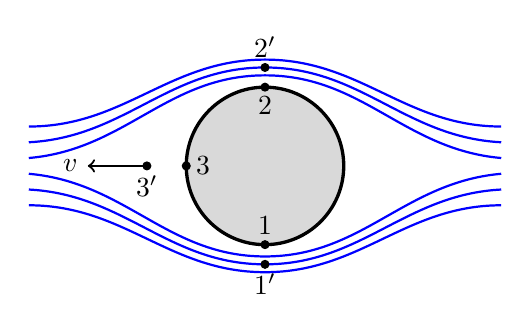
\begin{tikzpicture}
    \draw[very thick,fill=gray!30] (3,3) circle (1);
    \begin{scope}[yshift=0.1cm]
      \draw[blue,thick] (6,3) to[out=175,in=0] (3,4.05)
      to[out=180,in=5] (0,3); \draw[blue,thick] (6,3.2)
      to[out=177,in=0] (3,4.15) to[out=180,in=3] (0,3.2);
      \draw[blue,thick] (6,3.4) to[out=180,in=0] (3,4.25)
      to[out=180,in=0] (0,3.4);
    \end{scope}
    \begin{scope}[rotate around={180:(3,3)},yshift=0.1cm]
      \draw[blue,thick] (6,3) to[out=175,in=0] (3,4.05)
      to[out=180,in=5] (0,3); \draw[blue,thick] (6,3.2)
      to[out=177,in=0] (3,4.15) to[out=180,in=3] (0,3.2);
      \draw[blue,thick] (6,3.4) to[out=180,in=0] (3,4.25)
      to[out=180,in=0] (0,3.4);
    \end{scope}
    \draw[fill=black] (2,3) circle (0.05) node[right] {$3$};
    \draw[fill=black] (3,4) circle (0.05) node[below] {$2$};
    \draw[fill=black] (3,2) circle (0.05) node[above] {$1$};
    \draw[fill=black] (3,4.25) circle (0.05) node[above] {$2'$};
    \draw[fill=black] (3,1.75) circle (0.05) node[below] {$1'$};
    \draw[thick,->] (1.5,3) -- (0.75,3) node[left] {$v$};
    \draw[fill=black] (1.5,3) circle (0.05) node[below] {$3'$};
  \end{tikzpicture}
\end{center}


В точках 1 и 2 скорость воды $\approx 0$, а в точках 1' и 2'
находящихся чуть дальше от шарика, $V$. Сила вязкого трения, как
известно, равна $F = \eta S V /d$, следовательно, сила сопротивления
линейно зависит от скорости. 

Заметно, что перед шариком образуется <<водяная подушка>>, область
двигающейся вместе с шариком воды (область между точками 3 и
3'). Поток воды отражается от неё, изменяя импульс шарика: $\vec{F}
\Delta t = m \Delta \vec{V}$. 

\begin{center}
  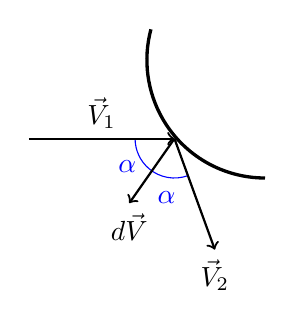
\begin{tikzpicture}
    \draw[very thick] (4,2) arc (270:165:1.5);

    \draw[blue] (2.85,2.5) ++(-70:0.5cm) arc (-70:-180:0.5cm);

    \draw[thick,->] (1,2.5) -- (2.85,2.5) node[midway,above] {$\vec{V}_1$}; 
    \draw[thick,->] (2.85,2.5) -- ++(-70:1.5cm) node[below] {$\vec{V}_2$};
    \draw[thick,->] (2.85,2.5) -- ++(-125:1cm) node[below] {$d\vec{V}$};
    
    \draw[blue] (2.75,1.75) node {$\alpha$};
    \draw[blue] (2.25,2.15) node {$\alpha$};
  \end{tikzpicture}
\end{center}

Рассмотрим отдельно взятый поток. Его начальная скорость равна
$\vec{V}_1$, конечная~---~$\vec{V}_2$. Так как площадь сечения воды
уменьшается, то $V_2 > V_1$, но незначительно, поэтому мы будем
считать, что $V_1 = V_2$. 

\begin{equation}
  \label{eq:bz_3}
  \vec{V}_1 + d\vec{V} = \vec{V}_2 \quad \Rightarrow \quad dV = V_1 (2 + 2 \cos
  \alpha). 
\end{equation}

При получении $\Delta \vec{V}_0 = \left(\int \Delta \vec{V}  dS \right)
/S$ перпендикулярные скорости шарика проекции взаимоуничтожаются (в
силу симметрии), а параллельные складываются, но все они
пропорциональны $V_1$, поэтому $\Delta V_0 \sim V_1$. 

Запишем закон изменения импульса: 

\begin{equation}
  \label{eq:bz_4}
  F = \frac{m \Delta V_0}{\Delta t} = \frac{S_{\mbox{ш}} V_1 \Delta t
    \rho \Delta V_0}{\Delta t} = S_{\mbox{ш}} \rho V_1 \Delta V_0 \quad
  \Rightarrow \quad F \sim V_1^2.
\end{equation}

Мы видим, что сила сопротивления пропорциональна квадрату скорости
набегающего потока. 

Кроме того, можно заметить, что на больших скоростях сзади шарика
появляется турбулентность, которая изменяет силу сопротивления. 

%%% Local Variables: 
%%% mode: latex
%%% TeX-master: "../../report"
%%% End: 
